\pdfminorversion=7
\documentclass[12pt]{article}

\usepackage{cmu-techreport}
\usepackage{listings}
\usepackage{color}
\usepackage{graphicx}

\definecolor{dkgreen}{rgb}{0,0.6,0}
\definecolor{gray}{rgb}{0.5,0.5,0.5}
\definecolor{mauve}{rgb}{0.58,0,0.82}

\lstset{frame=tb,
  language=Python,
  aboveskip=3mm,
  belowskip=3mm,
  showstringspaces=false,
  columns=flexible,
  basicstyle={\small\ttfamily},
  numbers=none,
  numberstyle=\tiny,
  keywordstyle=,
  commentstyle=\color{dkgreen},
  stringstyle=\color{mauve},
  breaklines=true,
  breakatwhitespace=true,
  tabsize=3
}

\title{STAT 608 Homework \#7}
\author{E. Lee Rainwater}
\date{11 July 2020}
\abstract{Use of genetic algorithm methods to select features for regression models.}

%\keywords{technical reports, typesetting, Carnegie Mellon University}

%\trnumber{CMU-CS-90-999}

%\citationinfo{\begin{center}
%To appear in a \TeX\ collection near you.
%\end{center}}

%\arpasupport{fox}
% \othersupport{the National Science Foundation under grant number 99-999-99}
% \authorsupport{The author holds a Froboz Gradual Fellowship.}

% \otherdisclaimer{NSF}



\makeatother

\usepackage{listings}
\renewcommand{\lstlistingname}{Listing}

\begin{document}
\maketitle

\section{Introduction}

The following general steps were used to evaluate various regression
methods and feature selection methods: 
\begin{enumerate}
\item Read, impute, and encode training \& validation data using\\
 \texttt{AdvancedAnalytics.ReplaceImputeEncode()}. 
\item Use a genetic algorithm as defined using the \texttt{DEAP} toolbox
to select features which provide the best fit of a \texttt{statsmodels}
ordinary least squares regression, as evaluated on the basis of \textit{Bayesian
Information Criterion} (BIC). 
\item Using the features selected by the genetic algorithm, generate a \texttt{statsmodel}
OLS model and validate it with holdout data, computing \textit{ASE}. 
\item Perform stepwise feature selection of the training data, generate
a \texttt{statsmodel} OLS model. Validate it with holdout data, computing
\textit{ASE}. 
\item Generate a \texttt{statsmodel} OLS model utilizing all features and
validate it with holdout data, computing \textit{ASE}. 
\item Perform a \textit{LASSO} regression utilizing predefined values of
the regularization parameter, $\alpha$. Use the features selected
by the \textit{LASSO} regression with the lowest \textit{BIC} to create
a validation model with the holdout data.
\end{enumerate}

\section{General Observations}

The fit results for the above models are presented in Table~\ref{tab:fit_summary}.

%\includegraphics{pasted1}
\begin{table}
    \caption{Summary of Model Fits}
    \label{tab:fit_summary}
    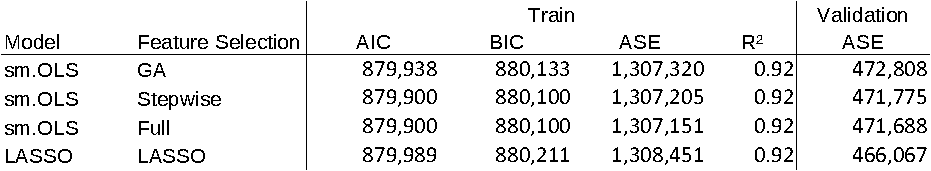
\includegraphics[width=\textwidth,height=\textheight,keepaspectratio]{table01-crop}
\end{table}

Of the models trained, the LASSO regression produced the model with
the lowest Validation Average Squared Error. 

\section{Appendix}

\subsection{Code Output}

\begin{verbatim}

**********************************************************************
********************** Loading attribute map... **********************
**********************************************************************

\end{verbatim}

\subsection{Code Listing}

{\tiny{}}
\begin{lstlisting}
def heading(headerstring):
    """
    Centers headerstring on the page. For formatting to stdout
    Parameters
    ----------
    headerstring : string
    String that you wish to center.
    Returns
    -------
    Returns: None.
    """
    tw = 70 # text width
    lead = int(tw/2)-(int(len(headerstring)/2))-1
    tail = tw-lead-len(headerstring)-2
    print('\n' + ('*'*tw))
    print(('*'*lead) + ' ' + headerstring + ' ' + ('*'*tail))
    print(('*'*tw))
    return
\end{lstlisting}
%{\tiny\par}
%
%{\tiny{}The title, authors, date, and technical report number will
%be typeset so as to be centered within the cut-out on the technical
%report cover page. If the material will not fit, you will get either
%an \verb+overfull \hbox+ message (if the material is too wide) or
%an \verb+overfull \vbox+ message (if the material is too long.) To
%create the title page, simply use \verb+\maketitle+ after \verb+\begin{document}+.}{\tiny\par}
%
%{\tiny{}In the interest of legibility technical reports should not
%be typeset at sizes below eleven point.}{\tiny\par}
\end{document}
